\documentclass{beamer}
\usepackage[utf8x]{inputenc}
\usepackage[english]{babel}
\usepackage{color}
\usepackage{soul}
\usepackage{mathtools}
\usepackage{graphicx}
\usepackage{mdframed}
\usepackage{marvosym}
\usepackage{tikz}
\usepackage{dirtytalk}
\usepackage{amsmath}
\usepackage{amssymb}% http://ctan.org/pkg/amssymb
\usepackage{pifont}
\usepackage{mathtools}
\usepackage{pdfpages}
\usepackage{float}
\usepackage{graphics}
\usepackage{color}
\usepackage{cancel}
\usepackage{graphicx} 
\usepackage{caption}
\usepackage[ruled,vlined]{algorithm2e}
\usepackage{tkz-graph}
\usepackage{tabularx}
\usepackage{multirow}
\usepackage{multicol}
\usepackage{csvsimple,booktabs,siunitx}
\usepackage{adjustbox}
\usepackage{xifthen}
\usepackage[normalem]{ulem}
\usepackage{xcolor}
\usepackage{changepage}
\usepackage{scrextend}
\usepackage{subfig}
\usepackage{booktabs,makecell}

\newcommand{\disc}[1]{{\color{blue}$\Rightarrow$\textbf{\textit{#1}}$\Leftarrow$}}
\newcommand{\cblue}[1]{{\usebeamercolor[fg]{structure} #1}}

\newcommand{\sample}[2]{#1^{(#2)}}
\newcommand{\cols}[4]{
	\begin{columns}[t]
	\begin{column}{#1\textwidth}
		#3
	\end{column}
	\begin{column}{#2\textwidth}
		#4
	\end{column}
	\end{columns}
	
}

\newcommand{\fig}[2]{
	\begin{figure}[!h]
	\includegraphics[scale=#1, draft=False]{#2}
	\end{figure}
}


%
% Choose how your presentation looks.
%
% For more themes, color themes and font themes, see:
% http://deic.uab.es/~iblanes/beamer_gallery/index_by_theme.html
%

\mode<presentation>
{
  \usetheme{default}      % or try Darmstadt, Madrid, Warsaw, ...
  \usecolortheme{default} % or try albatross, beaver, crane, ...
  \usefonttheme{default}  % or try serif, structurebold, ...
  \setbeamertemplate{navigation symbols}{}
  \setbeamertemplate{caption}[numbered]
  
} 


\setbeamertemplate{footline}
{
 \hbox{%
  \begin{beamercolorbox}[wd=.3\paperwidth,ht=2.7ex,dp=1ex,center]{author in head/foot}%
	\insertshortauthor
  \end{beamercolorbox}%
  \begin{beamercolorbox}[wd=.3\paperwidth,ht=2.6ex,dp=1ex,center]{author in head/foot}%
	{\usebeamercolor[fg]{footline} \insertshorttitle}
  \end{beamercolorbox}%
  \begin{beamercolorbox}[wd=.3\paperwidth,ht=2.6ex,dp=1ex,rightskip=.15cm, right]{author in head/foot}%
    \usebeamerfont{section in foot} \insertframenumber/\inserttotalframenumber
  \end{beamercolorbox}}%

  \vskip0pt%
}


\title[Data Mining]{Lecture 1: Introducing Data Mining Tools}

\author[CdLM Ing. Informatica a.a. 2018/2019]{Antonio Caliò}
\institute[]{\textit{DIMES, Università della Calabria} \\
87036 Rende (CS), Italia \\[1pt]
a.calio\MVAt dimes.unical.it}
%}

%}

\date{}


\begin{document}

\begin{frame}
  \titlepage
\end{frame}

\small
\begin{frame}{Key Concepts and Terminology}
\textsc{What is Data Mining?}\\
The term Data Mining refers to all the techniques whose goal
is to extract \underline{interesting}, \underline{non-trivial},
\underline{latent}, \underline{previously unknown} 
and {\usebeamercolor[fg]{structure} (hopefully) \textbf{useful}} information
from data.

\vskip 10pt
\begin{columns}[t]
\begin{column}{0.6\textwidth}
\textsc{Data vs Information}
\begin{table}
\scalebox{0.7}{
\begin{tabular}{c|c}
\hline
Name & Hair \\
\hline\hline
Orys Baratheon & black of hair \\
Axel Baratheon & black of hair \\
Lyonel Baratheon & black of hair \\
Steffon Baratheon & black of hair \\
Robert Baratheon & black of hair \\
\textbf{Joffrey Baratheon} & \textbf{golden-haired}
\end{tabular}
}
\end{table}
\pause
{\bf \color{red} Then, Joffrey is a ...}
\end{column}

\begin{column}{0.6\textwidth}
\textsc{The ``Knowledge Pipeline''}
\begin{figure}[!h]
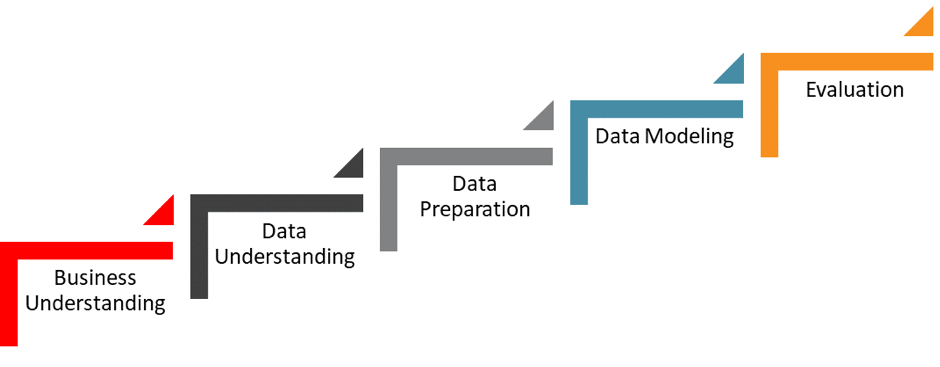
\includegraphics[scale=0.35]{img/pipe.png}
\end{figure}
\end{column}
\end{columns}

\end{frame}



\begin{frame}{Software \& Tools}
Here, the list of all the software, library and tools we are going to be familiar
with throughout this course.

\vskip 10pt
\begin{itemize}
\item \cblue{\underline{\textsc{Java-Based}}}
\begin{itemize}
\item[-] \textsc{Weka} - Data Mining Software in Java
\end{itemize}
\item \cblue{\underline{\textsc{Python-Based}}}
\begin{itemize}
\item[-] \textsc{scikit-learn} - Machine Learning in Python
\item[-] \textsc{NumPy} - Scientific Computation with Python
\item[-] \textsc{pandas} - Data Structures and Data Analysis tools
\item[-] \textsc{matplotlib} - Python 2D plotting library
\item[-] \textsc{seaborn} - Data Visualization library based on matplotlib with an
higher interface.
\end{itemize}
\item \cblue{\underline{\textsc{Jupyter}}} -
An open-source web application that allows you to create and share documents that contain live code, equations, visualizations and narrative text.
\end{itemize}
\end{frame}


\begin{frame}{}
\Huge
\centering
\cblue{Introduction to WEKA}
\end{frame}


\begin{frame}{What is Weka?}

\begin{minipage}[t]{.5\textwidth}
Weka stands for \textbf{\textsc{W}}aikato \textbf{\textsc{E}}nvironment for 
\textbf{\textsc{K}}nowledge
\textbf{\textsc{A}}nalysis; it is free an open-sources Data Mining workbench.
\end{minipage}
%
%
\hspace{0.3cm}
\begin{minipage}[t]{.3\textwidth}
\vspace{-0.5cm}
\begin{figure}[!t]

\includegraphics[scale=0.8]{img/logoWeka.png}
\end{figure}
\end{minipage}

\vskip 10pt
It provides a variety of machine learning algorithms for data mining tasks
\begin{itemize}
\item over 100 algorithms for classification tasks
\item 75 algorithms for data preprocessing
\item 25 algorithms for feature selection
\item 20 algorithms for unsupervised learning tasks
\end{itemize}

\vskip 10pt
It is developed and maintained by the University of Waikato, New Zealand.
\end{frame}

\begin{frame}{Download \& Installation}
Get WEKA from: \underline{\url{https://www.cs.waikato.ac.nz/ml/weka/}} 
(for Linux, Windows, Mac).
\vskip 10pt
\begin{columns}
\begin{column}{0.4\textwidth}
Select the latest stable version for your operating system and just run it
\end{column}
\begin{column}{0.7\textwidth}
\begin{figure}
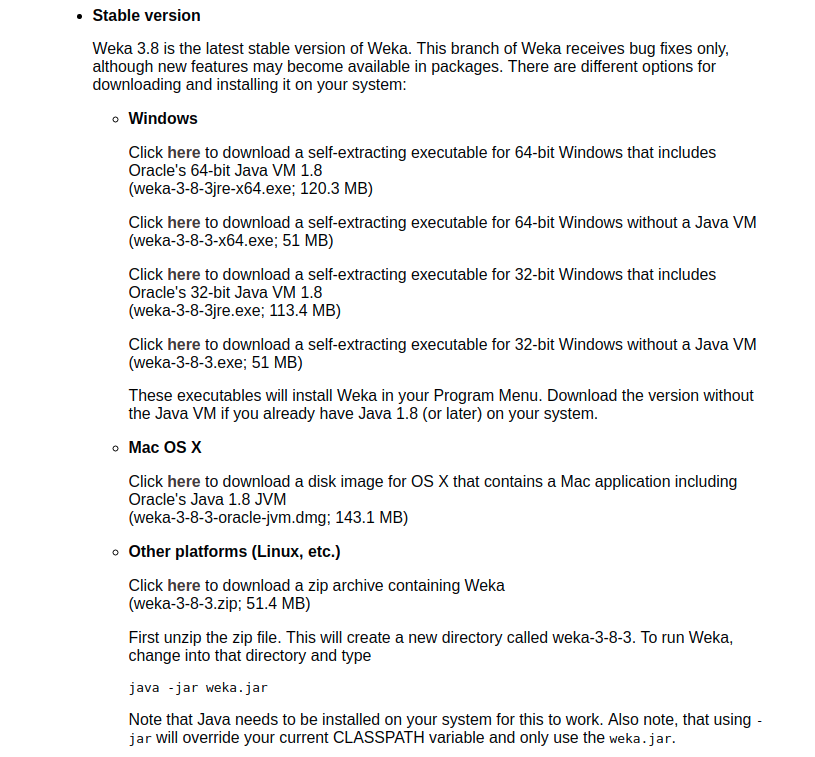
\includegraphics[scale=0.23]{img/download.png}
\end{figure}
\end{column}
\end{columns}
\end{frame}



\begin{frame}{Exploring the Explorer}
\cols{0.5}{0.5}{
 \cblue{\underline{\textsc{List of Tasks}}}\\
 Each tab on top of the window corresponds to a task.
 \begin{itemize}
 	\item[-] Preprocess: prepare your data
 	\item[-] Classify: execute a classification task
 	\item[-] Clustering: execute a clustering task
 	\item[-] Associate: find association rules
 	\item[-] Select Attributes: filter your data
 	\item[-] Visualize: visualize your data
 \end{itemize}
}
{
\fig{0.16}{img/tasks.png}
}
\end{frame}

\begin{frame}{Loading a Dataset}
Click on ``Open File''. 
Navigate to the WEKA installation directory
and go into the ``Data'' folder.
Here, you will find several datasets.

\fig{0.2}{img/data.png}


\vskip 0.5cm
For now, we will focus on the dataset named
``weather.nominal.arff''
\end{frame}

\begin{frame}[noframenumbering]{Analyzing the Data}
As the data are loaded, WEKA will present to you some basic
statistics on the loaded data.
\centering
\fig{0.5}{img/data_1.pdf}
\end{frame}

\begin{frame}[noframenumbering]{Analyzing the Data}
As the data are loaded, WEKA will present to you some basic
statistics on the loaded data.
\fig{0.5}{img/data_2.pdf}
\end{frame}

\begin{frame}[noframenumbering]{Analyzing the Data}
As the data are loaded, WEKA will present to you some basic
statistics on the loaded data.
\fig{0.5}{img/data_3.pdf}
\end{frame}


\begin{frame}[noframenumbering]{Analyzing the Data}
As the data are loaded, WEKA will present to you some basic
statistics on the loaded data.
\fig{0.5}{img/data_4.pdf}

\end{frame}

\begin{frame}{Take a peek at your data}
You can take a peek at your data by clicking on 
on the \textsc{Edit} button.
From this view, it is possible to modify your data. 
\cols{0.42}{0.7}{
\begin{itemize}
\item Adding a new instance/tuple
\item Removing a set of instances. You need to select
	  each instance you want to remove, right click on the selection and
	  then select ``Delete ALL selected instances'' from the drop down menu
\item Searching for a particular value
\item Modify a particular value
\end{itemize}
}{
\fig{0.2}{img/data.png}
}
\end{frame}

\begin{frame}{ARFF file}
An \cblue{ARFF} (Attribute-Relation File Format) file is an ASCII text file that describes a list of instances sharing a set of attributes.
ARFF files have two distinct sections. The first section is the \textbf{Header} information, which is followed the \textbf{Data} information.

The Header of the \cblue{ARFF} file contains the name of the relation, a list of the attributes (the columns in the data), and their types. 

An example header on the standard IRIS dataset looks like this:

\cols{0.5}{0.5}{

\begin{figure}
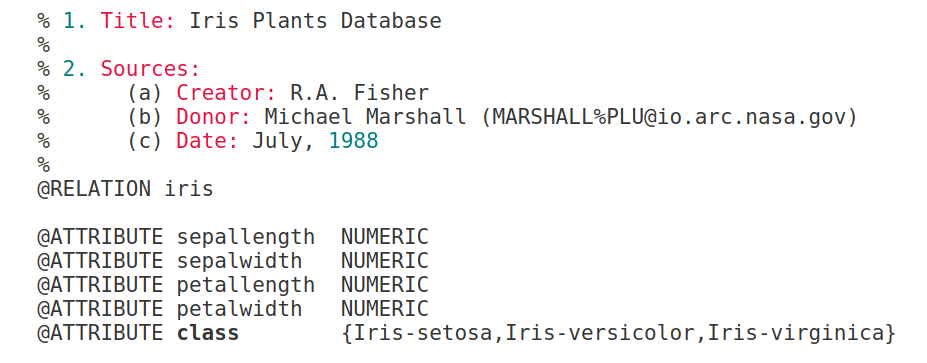
\includegraphics[scale=0.18]{img/arff_header.png}
\caption{\underline{\textsf{Header}}}
\end{figure}
}{
\begin{figure}
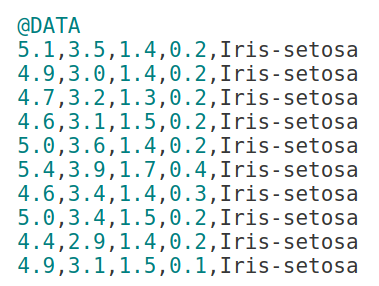
\includegraphics[scale=0.22]{img/arff_data.png}
\caption{\underline{\textsf{Data}}}
\end{figure}
}

\end{frame}


\begin{frame}[noframenumbering]{}
\Huge
\centering
\cblue{Filtering with WEKA}
\end{frame}

\begin{frame}{Filters}
Many machine learning algorithms are very sensitive to the input they are given. 
For this reason, knowing your data and preprocessing your dataset is a crucial task.\\[1pt]

Filters allow us to perform the following operations:
\begin{itemize}
\item \textsc{Data Cleaning}: fill in missing values, smooth noisy data,
identify or remove outliers
\item \textsc{Data Transformation}: normalization, standardization and aggregation
\item \textsc{Data Discretization}: replace numerical attributes with nominal ones
\end{itemize} 
Filters are divided into two categories: (i) \cblue{supervised} and (ii) \cblue{unsupervised} 
(most commonly used).\\[5pt]
Each of the aforementioned category includes two set of filters:
\begin{itemize}
\item[-] Instance Filters: they operate on the instances
\item[-] Attribute Filters: they operate on the attributes
\end{itemize}
\end{frame}

\begin{frame}{Sampling}
Sampling allows us to focus only on a limited portion of the whole dataset.
\vskip 0.2cm
{\color{red} But Why do we need to restrict ourselves to a limited portion?}
\pause
There are two main reasons:
\begin{itemize}
\item Gathering the whole dataset is too expensive
\item We cannot effort to execute the analysis on the whole dataset (e.g.,
we are in the earlier stages of our project).
\end{itemize} 
\pause
{\color{red} Which are the main pitfalls of sampling?}
\pause
When sampling we must be sure to extract a meaningful portion of the
data, i.e., the distribution of the extracted portion must reflect the one of
the entire dataset.
\cols{0.3}{0.8}{

\vspace{3mm}
In WEKA the sampling is done via the \textbf{ReservoirSample}}
{
\begin{figure}[t]
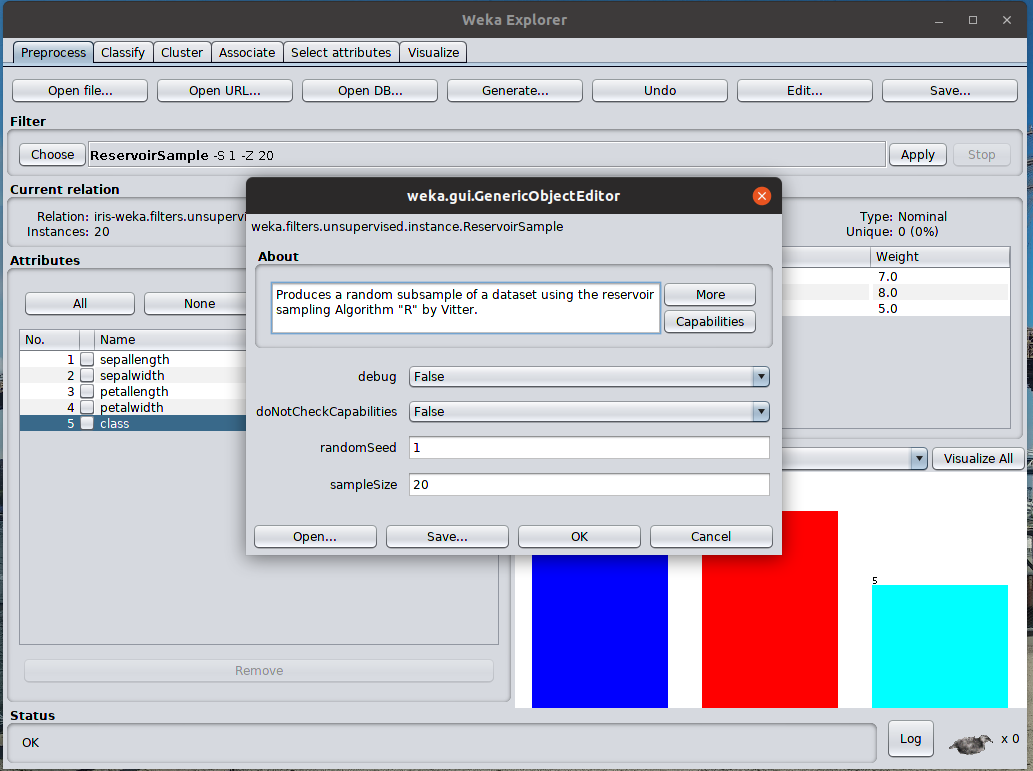
\includegraphics[scale=0.1]{img/sampling.png}
\end{figure}
}
\end{frame}

\begin{frame}[t]{Remove an Attribute}
{\color{red} Why do we need to remove some attribute?}
\pause
Several reasons:
\begin{itemize}
\item prevent the ``curse of dimensionality''
\item ease the data visualization
\item remove irrelevant and potentially redundant data
\end{itemize}

Select the \textbf{Remove Filter} under  \textsf{unsupervised filters/attribute filters}.

\centering
\begin{figure}
\begin{tabular}{lr}
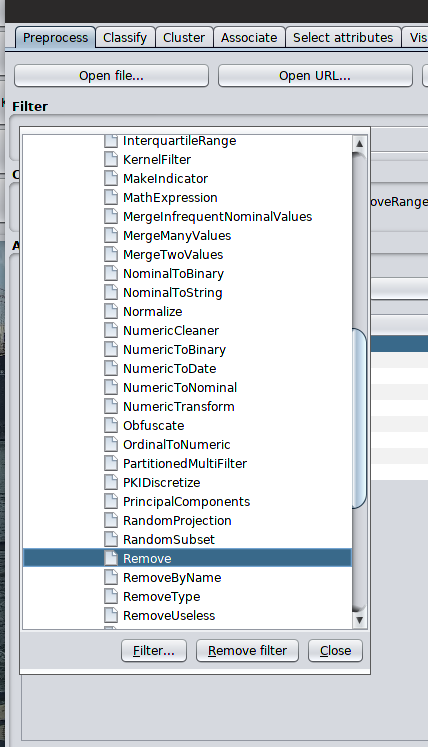
\includegraphics[scale=0.6]{img/remove.png} & 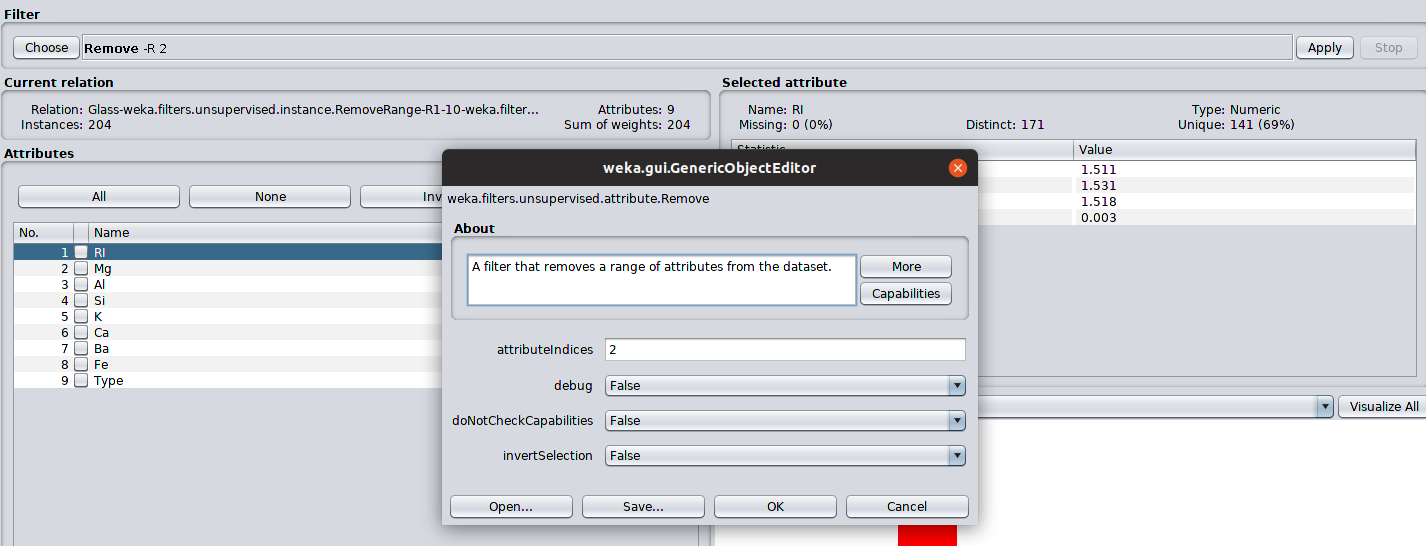
\includegraphics[scale=0.4]{img/remove2.png} \\
(a) Choose the filter & (b) filter configuration
\end{tabular}
\end{figure}
\end{frame}

\begin{frame}{Adding new Attributes}
We want to create new attributes by combining the information we already
have in the dataset.
\pause
{\color{red} Why do we need to combine different attributes?}
\pause
Let assume we have to solve a (silly) classification task. We need to
separate obese people from non-obese people. 
An useful indicator is the body mass index. We can derive this information
starting from the \textit{weight} and \textit{height}.
In this way we can inflate some a-priori knowledge inside the dataset.
\cols{0.5}{0.5}{

In WEKA, this is done via the \textbf{AddExpression}. 
It adds a new attribute, named according to 
\textit{name} field of the form, whose value are obtained
computing the given formula. For instance, $a1+a2$
set the values of the new attribute as the sum of the first and second
columns.
}
{
\begin{figure}[t]
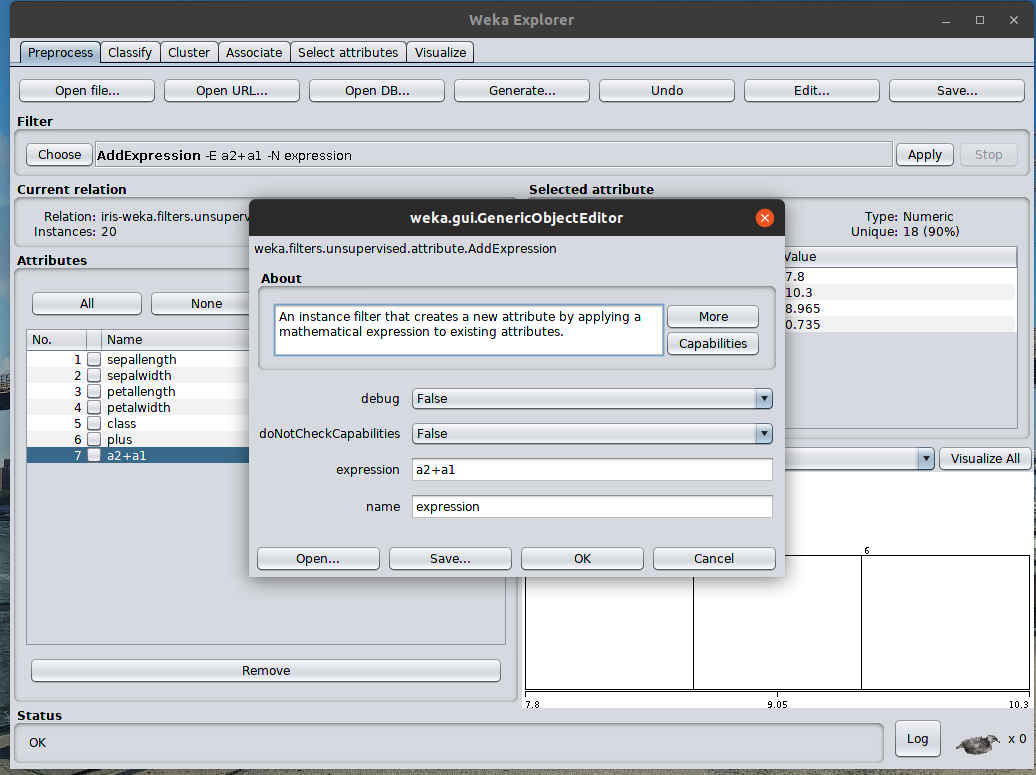
\includegraphics[scale=0.12]{img/add.png}
\end{figure}
}
\end{frame}

\begin{frame}{Normalization}
We want our data to be inside a given interval (usually $[0,1]$). 
Therefore each instance is transformed s.t.
\[
	x' = \frac{x-Min}{Max-Min}(Max_{range}-Max_{range})+Min _{range}
\]
\cols{0.5}{0.5}{

In WEKA, this is done via the \textbf{Normalize}.
By default this filter normalize all the data in the range
$[0,1]$. 

}
{
\begin{figure}[t]
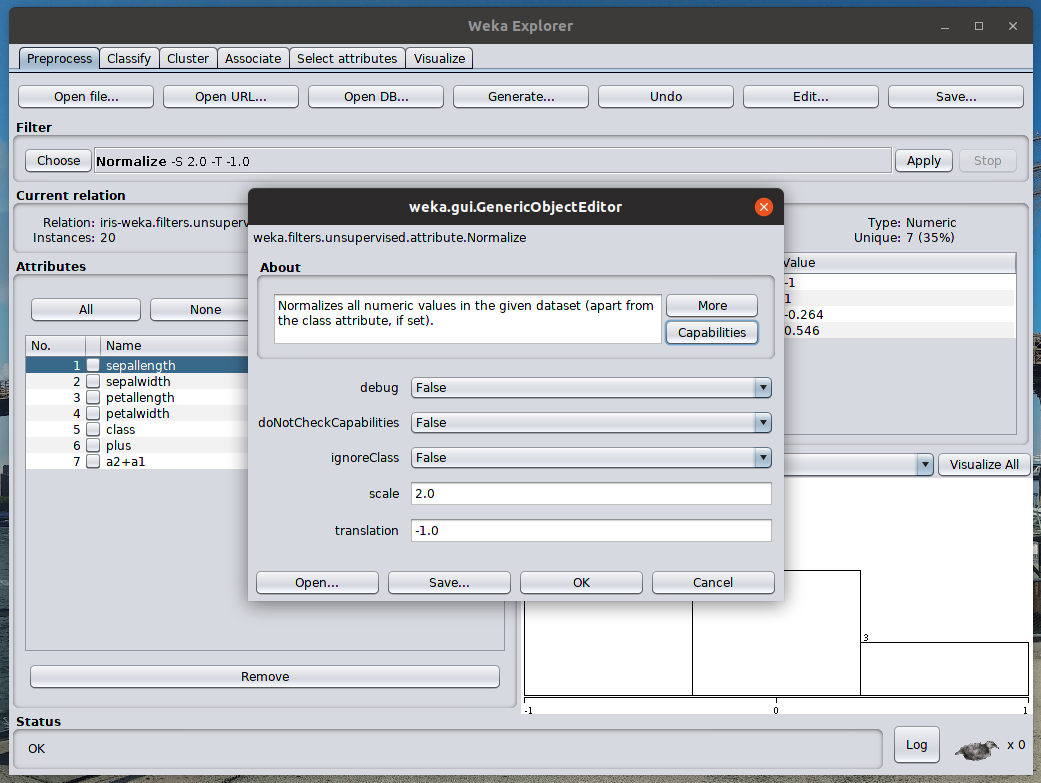
\includegraphics[scale=0.12]{img/normalize.png}
\end{figure}
}
\end{frame}

\begin{frame}{Standardization}
The Standardization (or Z-score normalization) 
transform the data in order to fit a normal distribution
$\mathcal{N}(0,1)$, i.e., a normal distribution with
mean 0 and standard deviation 1.
\[
	x' = \frac{x-\mu(A)}{\sigma(A)}
\]
Where $\mu(A)$ (resp. $\sigma(A)$)
is the mean (resp. standard deviation) computed with respect to the
attribute A.
\cols{0.5}{0.5}{

In WEKA, this is done via the \textbf{Standardize}.
}
{
\begin{figure}[t]
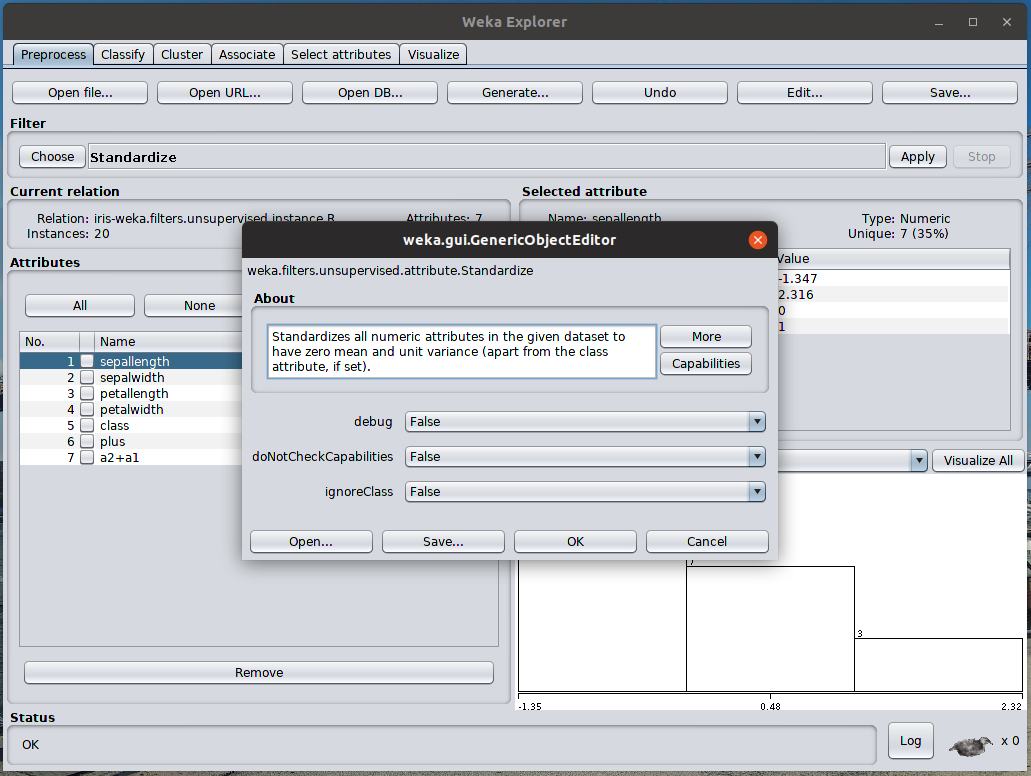
\includegraphics[scale=0.12]{img/standardize.png}
\end{figure}
}
\end{frame}





\begin{frame}[t]{Discretize an Attribute}
Select the Discretize Filter under the \textsf{unsupervised filters -> attribute filters}.
\cols{0.5}{0.5}{
	The most important parameter is the number of different bins we want to split
	the selected attribute. By default, WEKA will divide the entire span of values
	of the selected attribute in 10 bins.\\
	After the filter has done, each instance will be assigned with a label corresponding
	to the interval such instance falls back into (w.r.t to the selected attribute)
	
}
{
\fig{0.8}{img/discrete.png}
}
\end{frame}

\begin{frame}{Multiple Filters}
It we choose \textit{MultiFilter} from the dropdown menu, WEKA will
show the following interface. 
\begin{figure}
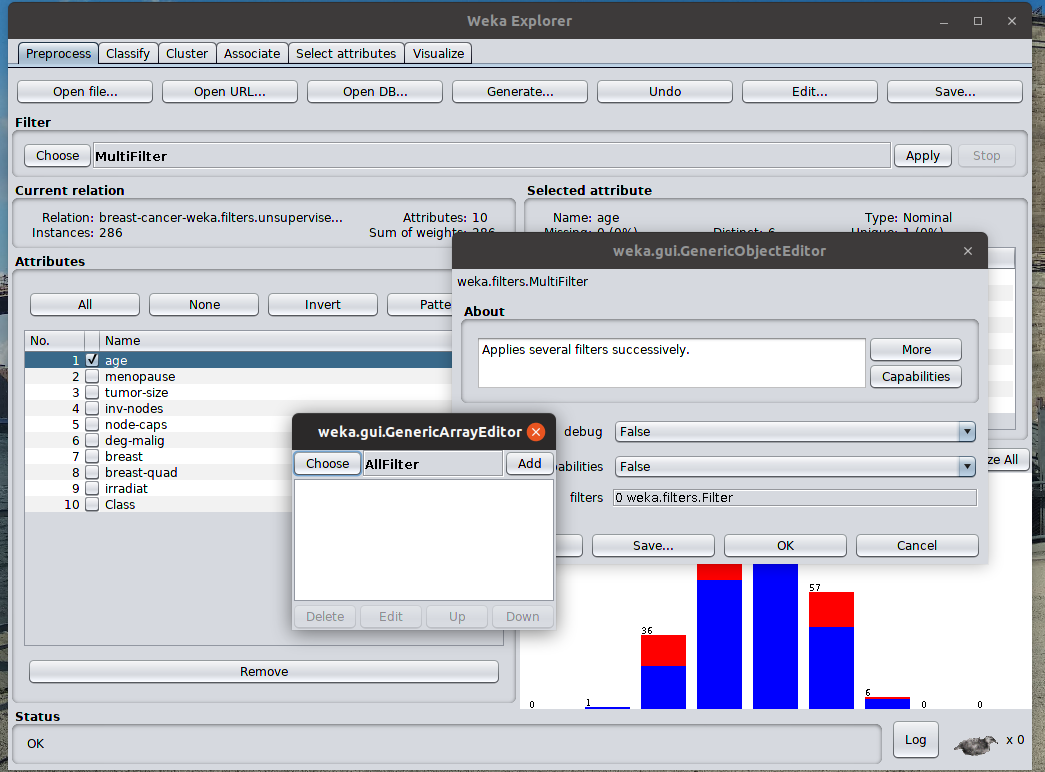
\includegraphics[scale=0.2]{img/chain.png}
\end{figure}
Here, we can define a chain of filters, which will be applied one after the
other.
\end{frame}

\begin{frame}[t]{Removing Null Instances}
One way of dealing with null instances is to remove
the instances with missing values.
\vskip 0.3cm
\cols{0.35}{0.7}{
In WEKA, this can be done with the
\textbf{SubsetByExpression} filter.
It we set in the expression field ``\textsc{not is missing(a2)}''
WEKA will retrieve all the data that match the given expression.
}
{
\fig{0.2}{img/missing_null.png}
}
\end{frame}

\begin{frame}{Dealing with Null Instances}
If we have several missing values the best way to deal with this situation is
to replace the missing values rather than removing the entire corresponding instance
\vskip 0.3cm
\cols{0.3}{0.7}{
In WEKA, this is done via the \textbf{ReplaceMissingValue} filter. 
By default, WEKA will replace the missing value with the mean
associated with the attribute.
}
{
\begin{figure}
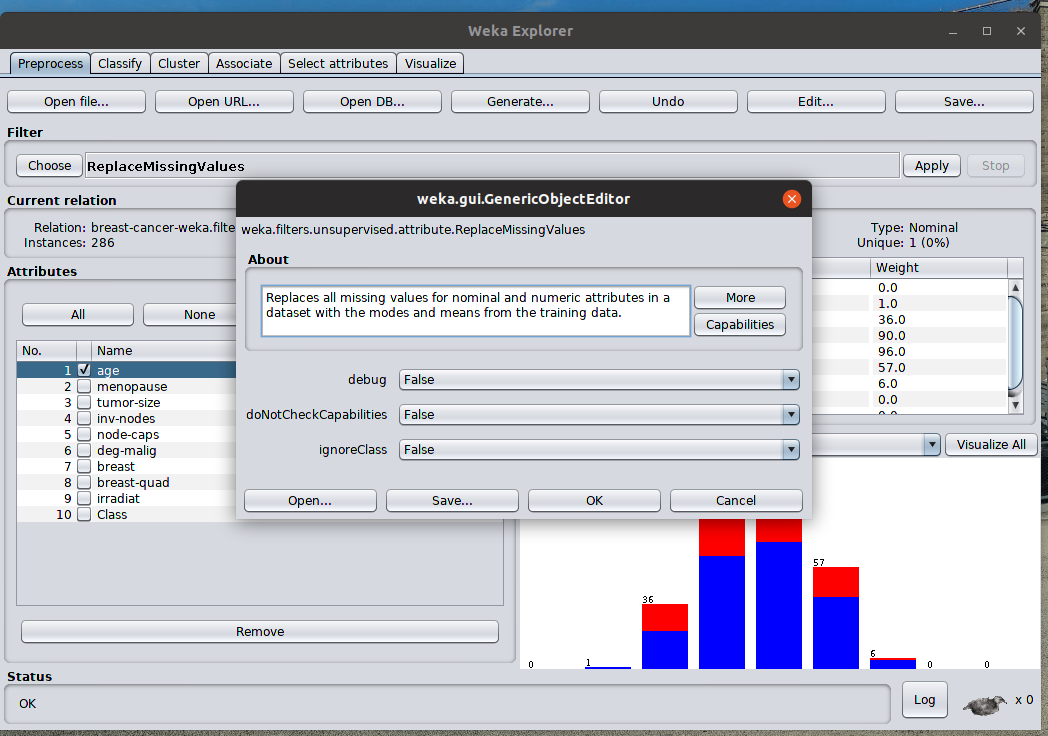
\includegraphics[scale=0.2]{img/missing.png}
\end{figure}
}

\end{frame}


\begin{frame}[noframenumbering]{}
\Huge
\centering
\cblue{Visualizing with WEKA}
\end{frame}

\begin{frame}{Visualize}
Load the \textsf{iris.arff} dataset\\[5pt]
Open the visualize tab.  WEKA will present a grid which consists
of several 2-dimensional scatter plots, obtained by combining each attribute
with the others.\\[5pt]
\cols{0.5}{0.6}{
By clicking on a particular plot, WEKA opens a restricted view on the selected graph.\\[5pt]
From this view we can manipulate the axes, by choosing a different combination attributes
for the x and the y axis.\\
Each point is represented with the color corresponding to its class
}{
\fig{0.5}{img/visualize.png}
}

\end{frame}


\begin{frame}[noframenumbering]{}
\Huge
\centering
\cblue{Classification with WEKA}
\end{frame}


\begin{frame}{What is the Classification Problem?}
We are given with a set of samples in the form $\langle \sample{x}{i}, \sample{y}{i} \rangle$, where $\sample{x}{i}$ is the features-vector
associated with the $i$-th instance in our dataset and $\sample{y}{i}$ is
categorical value with denotes the class the $i$-th instance belongs to
\vskip 10pt
\begin{mdframed}[backgroundcolor=blue!30] 
The Classification Problem asks to correctly assign a label, i.e, a class, to
any previously unseen sample
\end{mdframed}
\pause
\vspace{0.5cm}
\cblue{\textsf{Example}}-To which house does this character belong to?
\cols{0.5}{0.5}{
\fig{0.7}{img/dany.jpg}
}
{
\begin{table}
\begin{tabular}{c|c}
\textsc{Attribute} & \textsc{Value} \\
\hline
 Hair & Silver \\
 Skin & Pale \\
 Eyes & Light Blue \\
 Mother Tongue & Valyrian \\
  Age & 21 \\
 Height & 1.72 \\
 \hline 
\color{red}{House} & \color{red}{\textbf{???????}} \\
 \hline
\end{tabular}
\end{table}
}
\end{frame}

 
\begin{frame}[noframenumbering]{What is the Classification Problem?}
We are given with a set of samples in the form $\langle \sample{x}{i}, \sample{y}{i} \rangle$, where $\sample{x}{i}$ is the features-vector
associated with the $i$-th instance in our dataset and $\sample{y}{i}$ is
categorical value with denotes the class the $i$-th instance belongs to
\vskip 10pt
\begin{mdframed}[backgroundcolor=blue!30] 
The Classification Problem asks to correctly assign a label, i.e, a class, to
any previously unseen sample
\end{mdframed}

\vspace{0.5cm}
\cblue{\textsf{Example}}-To which house does this character belong to?
\cols{0.5}{0.5}{
\fig{0.7}{img/dany.jpg}
}
{
\begin{table}
\begin{tabular}{c|c}
\textsc{Attribute} & \textsc{Value} \\
\hline
 Hair & Silver \\
 Skin & Pale \\
 Eyes & Light Blue \\
 Mother Tongue & Valyrian \\
 Age & 21 \\
 Height & 1.72 \\
 \hline 
\color{red}{House} & \color{red}{\textbf{Targaryen}} \\
 \hline
\end{tabular}
\end{table}
}
\end{frame}
 
 
 
 
\begin{frame}[t]{Get your hands dirty}

Open the \underline{\textsf{glass.arff}} file.
\cols{0.4}{0.7}{

Attributes:
\begin{itemize}
\item[-] \textsc{RI}: reflecting index
\item[-] \textsc{Na}: Sodium
\item[-] \textsc{Mg}: Magnesium
\item[-] \textsc{K}: Potassium
\item[-] \textsc{Ca}: Calcium
\item[-] \textsc{Ba}: Barium
\item[-] \textsc{Fe}: Iron
\item[-] \textsc{Type of glass}
\end{itemize}
}{
\fig{0.2}{img/glass.png}
}
\end{frame}


\begin{frame}{Select a Classifier}
Open the ``Classify'' tab. Press on the ``Choose'' button and then select
the \textsf{J48} classifier

\fig{0.5}{img/classify.pdf}
\end{frame}

\begin{frame}{Output}
When the training is done, WEKA presents some information about
the classifier. Such as:
\cols{0.5}{0.5}{

\textsc{Summary}\\
\tiny
\begin{table}
\begin{tabular}{l@{\hspace{0.8mm}}l@{\hspace{-0.5mm}}l}
Correctly Classified Instances     &     42       &        57.5342 \\
Incorrectly Classified Instances   &    31         &      42.4658 \\
Kappa statistic                    &      0.4259 & \\
Mean absolute error                &      0.1246 & \\
Root mean squared error            &      0.3287 & \\
Relative absolute error            &     58.7442 & \\
Root relative squared error        &    101.8335 & \\
Total Number of Instances          &     73     & \\
\end{tabular}
\end{table}
}
{

\textsc{Confusion Matrix}
\tiny
\begin{table}

\begin{tabular}{c@{\hspace{1.2mm}}c@{\hspace{1.2mm}}c@{\hspace{1.2mm}}c@{\hspace{1.2mm}}c@{\hspace{1.2mm}}c@{\hspace{1.2mm}}c|l}
  a & b & c & d & e & f & g &  classified as \\
  \hline
 12 & 6 & 1 & 0 & 0 & 0 & 1 & a = build wind float \\
  7 &16 & 1 & 0 & 2 & 3 & 3 & b = build wind non-float \\
  2 & 0 & 1 & 0 & 0 & 0 & 1 & c = vehic wind float \\
  0 & 0 & 0 & 0 & 0 & 0 & 0 & d = vehic wind non-float \\
  0 & 0 & 0 & 0 & 2 & 0 & 2 & e = containers \\
  1 & 0 & 0 & 0 & 0 & 1 & 0 & f = tableware \\
 1 & 0 & 0 & 0 & 0 & 0 & 10 & g = headlamps 
\end{tabular}
\end{table}

}
\textsc{Detailed Accuracy by Class}
\tiny
\vspace{-0.5cm}
\begin{table}
\scalebox{0.9}{
\begin{tabular}{llllllllll}
                 TP Rate & FP Rate & Precision & Recall &  F-Measure & MCC    &  ROC Area & PRC Area & Class \\
                 0,600  &  0,208   & 0,522   &   0,600  &  0,558    &  0,377  &  0,727   &  0,482   &  build wind float \\
                 0,500   & 0,146  &  0,727   &   0,500  &  0,593    &  0,382  &  0,669   &  0,564   &  build wind non-float \\
                 0,250   & 0,029  &  0,333   &   0,250  &  0,286    &  0,253  &  0,817   &  0,393   &  vehic wind float \\
                 ?      &  0,000  &  ?       &   ?      &  ?        &  ?      &  ?       &  ?       &  vehic wind non-float \\
                 0,500  &  0,029  &  0,500   &   0,500  &  0,500    &  0,471  &  0,947   &  0,445   &  containers \\
                 0,500 &   0,042   & 0,250   &   0,500  &   0,333   &   0,328  &  0,729  &   0,139  &   tableware \\
  0,909  &  0,113  &  0,588   &   0,909  &  0,714    &  0,674  &  0,905   &  0,582   &  headlamps \\
 0,575  &  0,142 &   0,603   &   0,575  &  0,572    &  0,421 &   0,746   &  0,517   &  \underline{Weighted Avg.} 
\end{tabular}
}
\end{table}
\end{frame}




\iffalse
\begin{frame}{What is Machine Learning?}
\huge
The term ``Machine Learning''  refers to all the \textit{algorithms} and 
\textit{techniques} that allow us to infer some hidden knowledge directly from data.
\end{frame}

\begin{frame}{Different Classes of ML Problems}
\large
We can devise three different classes of machine learning problems:
\begin{itemize}
\item \textsc{Supervised Learning}
Is the task of learning a function that maps an input to and output w.r.t. a set of
pair $\langle$ input, output $\rangle$.  
\iffalse
Supervised learning is the machine learning task of learning a function that maps an input to an output based on example input-output pairs.[1] It infers a function from labeled training data consisting of a set of training examples.[2] In supervised learning, each example is a pair consisting of an input object (typically a vector) and a desired output value (also called the supervisory signal). A supervised learning algorithm analyzes the training data and produces an inferred function, which can be used for mapping new examples. An optimal scenario will allow for the algorithm to correctly determine the class labels for unseen instances. This requires the learning algorithm to generalize from the training data to unseen situations in a "reasonable" way (see inductive bias).
\fi

	\begin{itemize}
    	\item Regression - The output is a numerical property
        \item Classification - The output is a binary (or categorical) property
    \end{itemize}

\item \textsc{Unsupervised Learning} 
Is the task of learning hidden structural properties from ``unlabeled'' data
\iffalse
Unsupervised machine learning is the machine learning task of inferring a function to describe hidden structure from "unlabeled" data (a classification or categorization is not included in the observations). Since the examples given to the learner are unlabeled, there is no evaluation of the accuracy of the structure that is output by the relevant algorithm—which is one way of distinguishing unsupervised learning from supervised learning and reinforcement learning.

A central case of unsupervised learning is the problem of density estimation in statistics,[1] though unsupervised learning encompasses many other problems (and solutions) involving summarizing and explaining key features of the data.
\fi
	\begin{itemize}
		\item Clustering 
	\end{itemize}
\item \textsc{Reinforcement Learning} is the task of learning by trials
\end{itemize}
\end{frame}


\begin{frame}{Different Classes of ML Problems}
\large
We can devise three different classes of machine learning problems:
\begin{itemize}
\item \textsc{Supervised Learning}
Is the task of learning a function that maps an input to and output w.r.t. a set of
pair $\langle$ input, output $\rangle$.  
\iffalse
Supervised learning is the machine learning task of learning a function that maps an input to an output based on example input-output pairs.[1] It infers a function from labeled training data consisting of a set of training examples.[2] In supervised learning, each example is a pair consisting of an input object (typically a vector) and a desired output value (also called the supervisory signal). A supervised learning algorithm analyzes the training data and produces an inferred function, which can be used for mapping new examples. An optimal scenario will allow for the algorithm to correctly determine the class labels for unseen instances. This requires the learning algorithm to generalize from the training data to unseen situations in a "reasonable" way (see inductive bias).
\fi

	\begin{itemize}
    	\item Regression - The output is a numerical property
        \item Classification - The output is a binary (or categorical) property
    \end{itemize}

\item \textsc{Unsupervised Learning} 
Is the task of learning hidden structural properties from ``unlabeled'' data
\iffalse
Unsupervised machine learning is the machine learning task of inferring a function to describe hidden structure from "unlabeled" data (a classification or categorization is not included in the observations). Since the examples given to the learner are unlabeled, there is no evaluation of the accuracy of the structure that is output by the relevant algorithm—which is one way of distinguishing unsupervised learning from supervised learning and reinforcement learning.

A central case of unsupervised learning is the problem of density estimation in statistics,[1] though unsupervised learning encompasses many other problems (and solutions) involving summarizing and explaining key features of the data.
\fi
	\begin{itemize}
		\item Clustering 
	\end{itemize}
\item \textsc{Reinforcement Learning} is the task of learning by trials
\end{itemize}
\vskip 0.8cm
\huge
\textcolor{red}{We will only deal with supervised learning problem!}
\end{frame}


\begin{frame}{Supervised Learning: A big Picture}
\begin{center}
\includegraphics[scale=0.6]{img/supervised_learning.pdf}
\end{center}
\end{frame}

\begin{frame}{Terminology: Dataset, Features and Labels}
\Large
\begin{itemize}
	\item \textsc{Dataset} -  A collection of \textit{examples} 
    \item \textsc{Example} - One row of a data set. An example contains one or more features.
    	It can be either a labeled example or an unlabeled example
    \item \textsc{Feature} - An input variable used in making predictions
    \item \textsc{Label} - In supervised learning, the ``answer" or ``result" portion of an example
\end{itemize}

\end{frame}

%%%%%%%%%%%%%%%%%%%%%%
% Linear Regression  %
%%%%%%%%%%%%%%%%%%%%%%
\section{Linear Regression}
\begin{frame}
\tableofcontents[currentsection]
\end{frame}

\begin{frame}{Let's start with an example}
\small
We are given with a dataset representing the living area and prices
of a set of houses from Cosenza.

\begin{table}
\begin{tabular}{c|c}
Living Area (m$^2$) & Price (\$) \\ 
\hline
95 & 105.000 \\
60 & 85.000 \\
 . & . \\
 . & . 
\end{tabular}
\end{table}

\begin{columns}
\begin{column}{0.5\textwidth}
\includegraphics[scale=0.4]{img/Initial.pdf}
\end{column}
\begin{column}{0.5\textwidth}
\iffalse
We need to find the straight line that best captures
the linear relation between \textit{Living Area} and \textit{Price}.
\[
	f(x) \simeq h(x) = w \cdot x + b
\]
\fi
\end{column}
\end{columns}
\end{frame}


\begin{frame}{Let's start with an example}
\small
We are given with a dataset representing the living area and prices
of a set of houses from Cosenza.

\begin{table}
\centering
\begin{tabular}{c|c}
Living Area (m$^2$) & Price (\$) \\ 
\hline
95 & 105.000 \\
60 & 85.000 \\
 . & . \\
\end{tabular}
\end{table}
\begin{columns}
\begin{column}{0.5\textwidth}
\includegraphics[scale=0.3]{img/line.pdf}

\end{column}
\begin{column}{0.5\textwidth}
We need to find the straight line that best captures
the linear relation between \textit{Living Area} and \textit{Price}.
\[
	f(x) \simeq h(x) = w \cdot x + b
\]

\end{column}
\end{columns}
\pause
There are several way of fitting a line through the points.
The question is: \underline{Which is the best one?}\\
\pause
We need  way of measuring how good we are fitting the data
\end{frame}


\begin{frame}{Loss Function}
It tells how good we are fitting the data. \\
We are actually measuring the red lines in the graph.
\vskip 1cm
\begin{columns}
\begin{column}{0.5\textwidth}
\includegraphics[scale=0.4]{img/ErrorBar.pdf}
\end{column}
\begin{column}{0.5\textwidth}
Two of the most common loss functions are:
\begin{itemize}
\item \textsc{Least Square (L$_2$)}
		\[
        	L_2 = \sum_{i}^{N} (h(\sample{x}{i}) - \sample{y}{i})^2
        \]
\item \textsc{Mean Least Square (MLS)}
		\[
        	MLS = \frac{1}{N} \sum_{i}^{N} (h(\sample{x}{i}) - \sample{y}{i})^2
        \]
\end{itemize}
\end{column}
\end{columns}
\end{frame}

\begin{frame}{Take a deep breath!}
\textsc{Input:} A dataset. Each sample is in the form $\langle \sample{x}{i}, \sample{y}{i} \rangle$ \\
\vskip 0.8cm
\textsc{Objective:} Find a linear relationship between the features ($\sample{x}{i}$) and the labels ($\sample{y}{i}$).\\
This linear relationship will eventually allow us to predict the value of $y$ on previously unseen data
\vskip 0.8cm
\textsc{Problem:} After defining a \textit{loss function} we are left with the task of minimizing such function.\\
\vskip 1cm
\pause
\huge
\textcolor{red}{How can we?}
\pause
\textcolor{red}{\underline{The Gradient Descent Algorithm}} 
\end{frame}


%%%%%%%%%%%%%%%%%%%%%%%%%
%     REDUCING LOSS     %
%%%%%%%%%%%%%%%%%%%%%%%%%
\section{Reducing Loss}
\begin{frame}
\tableofcontents[currentsection]
\end{frame}

\begin{frame}[fragile]{An iterative approach}
Here is an overview of the gradient descent algorithm
\vskip 0.8cm
	\centering
	\includegraphics[scale=0.3]{img/iterative_approach.png}
\end{frame}

\begin{frame}{Digression: From Derivative to the Gradient}
\scriptsize
\textsc{Derivative}\\
The derivative of a function measures the sensitivity to change of the function value (output value) with respect to a change in its argument (input value).\\
Given a function $y=f(x)$, its derivative in a particular point $x_0$ is
the slope of the tangent line to the graph of the function at that point. 
\vskip 0.2cm
\textsc{Directional Derivative}\\
The directional derivative of a multi-variable function
along a given vector $v$ at a given point $x$ intuitively represents the instantaneous rate of change of the function, moving through $x$
along the direction specified by vector $v = \langle v_1, v_2 \rangle$.\\
The directional derivative is denoted with:
\[\frac{\partial f(x_1,x_2)}{\partial v} = \lim_{t \to 0} \frac{f(x_1+t \cdot v_1,x_2+t \cdot v_2)}{t}\] 
A \textit{partial derivative} is a specialization of the directional
derivative where the vector $v$ belongs to canonical basis of the function space.
\vskip 0.2cm
\textsc{Gradient}\\
The gradient is no more than a vector containing all the partial derivatives
w.r.t. each variable. It is denoted with the symbol $\nabla f(\cdot)$
	
The gradient points in the direction of the greatest rate of increase of the function, and its magnitude is the slope of the graph in that direction. 
\end{frame}


\begin{frame}{Gradient Descent: a Visual Introduction}
\begin{columns}
\begin{column}{0.6\textwidth}
\includegraphics[scale=0.6]{img/gradientalgorithm.pdf}
\end{column}
\begin{column}{0.5\textwidth}
\begin{itemize}
\pause
\item Randomly select an initial assignment for the model weights
\pause
\item Compute the gradient of the loss function w.r.t. the weights
\pause
\item Reassign the model weights according to the update rule
\end{itemize}
\pause 
\large
\textcolor{red}{WTF is the update rule?} \\
\textcolor{red}{(negative) gradient tells us the direction of the steepest decrease in the loss
function, it does not tell us how much we can follow such direction!}
\end{column}
\end{columns}
\end{frame}


\begin{frame}{Gradient Descent: the Learning Rate}
Iteration after iteration all the weights of the model are updated according to the
following \textit{update rule}:
\[
	w_{j}^{i+1} = w_{j}^{i} - \alpha \frac{\partial}{\partial_j} L(W) \text{,  (w.r.t. a set of data points)}
\]
$L(\cdot)$ is the loss function.\\
\vskip 0.5cm
Choosing the learning rate is a crucial task. We can devise two extremes cases.
\vskip 0.5cm
\begin{columns}
\begin{column}{0.5\textwidth}
\underline{$\alpha$ is too small}
\includegraphics[scale=0.4]{img/toosmall.pdf}
\end{column}
\begin{column}{0.5\textwidth}
\underline{$\alpha$ is too big}
\includegraphics[scale=0.4]{img/toobig.pdf}
\end{column}
\end{columns}
\end{frame}




\begin{frame}{Gradient Descent: Batch Size}
In Gradient Descent the term \textbf{batch} refers to the number of points used to calculate the
gradient in a single iteration of the algorithm. \\
We can define three different versions of the algorithm, based on the batch size
\vskip 1cm
\begin{itemize}
\item \textsc{Batch Gradient Descent}
\item \textsc{Stochastic Gradient Descent}
\item \textsc{Mini-Batch Stochastic Gradient Descent}
\end{itemize}
\end{frame}

\begin{frame}{Batch Gradient Descent (BGD)}
\large
Each iteration computes the gradient w.r.t. all the points in the dataset.
\vskip 0.5cm
\begin{center}
\begin{algorithm}[H]
 \Repeat{convergence}{
 $w_{j}^{i+1} = w_{j}^{i} - \alpha \sum_{i} \frac{\partial}{\partial_j} L(W)$ (for every j)\;
}
\end{algorithm}
\end{center}
\pause
\begin{itemize}
\item \textsc{PROS:} We only need to compute the gradient once
\pause
\item \textsc{CONS:} If the batch is too large, computing the gradient will need a huge amount of time
\end{itemize}
\end{frame}

\begin{frame}{Stochastic Gradient Descent (SGD)}
We settle for an estimate of the actual gradient by computing its average.\\
We sample uniformly at random just one sample at each iteration and then we compute
the gradient w.r.t. such point.
\begin{center}
\begin{algorithm}[H]
\DontPrintSemicolon
 \Repeat{convergence}{
  select a point $\sample{x}{i}$ uniformly at random from the dataset\;
  
  $w_{j}^{i+1} = w_{j}^{i} - \alpha \frac{\partial}{\partial_j} L(W)$ (for every j w.r.t. $\sample{x}{i}$)\;

}
\end{algorithm}
\end{center}

\pause
\begin{itemize}
\item \textsc{PROS:} It is often much faster than the batch gradient descent. Each iteration takes less time
\pause
\item \textsc{CONS:} It is too sensitive to noisy data. It may never converge to the minimum (but it is unlikely)
\end{itemize}

\end{frame}

\begin{frame}{mini-Batch Stochastic Gradient Descent (mBGD)}
It is a tradeoff between the efficiency of SGD and the effectiveness of BGD. \\
The gradient is computed w.r.t. a batch of size between 10 and 1.000 examples

\begin{center}
\begin{algorithm}[H]
\DontPrintSemicolon
 Let k be the number of points in each batch\;
 \Repeat{convergence}{
  
  select $k$ points uniformly at random from the dataset\;
  
  $w_{j}^{i+1} = w_{j}^{i} - \alpha \frac{\partial}{\partial_j} L(W)$ (for every j w.r.t. $\sample{x}{i}$)\;
}
\end{algorithm}
\end{center}
\end{frame}

\begin{frame}{Recap}
We have introduced the gradient descent procedure for minimizing the loss function.\\
\vskip 0.5cm
Among the three different versions \textit{mBGD} is the most used. \\

\vskip 1cm
There are two important parameters to specify:
\begin{itemize}
\pause
\item Learning Rate ($\alpha$). If $\alpha$ is too small then the algorithm will take ages before reaching the convergence.
	  If $\alpha$ is too high then the algorithm will be unstable, we will also loose the guarantee of reaching the global minimum of the loss function
\pause      
\item Batch Size ($k$). If $k$ is too small then the algorithm will be more sensitive to noisy data. If $k$ is too big each iteration will take longer
\end{itemize}
\end{frame}


%%%%%%%%%%%%%%%%%%%%%%%%
%    Generalization    %
%%%%%%%%%%%%%%%%%%%%%%%%
\section{Generalization}
\begin{frame}
\tableofcontents[currentsection]
\end{frame}

\begin{frame}{Model Performance}
\Large
How can we evaluate if the model has been well trained?
There are two main measures we have to consider to important quantities:
\vskip 0.8cm
\begin{itemize}
\item In-Sample Error ($E_{in}$). It tells how good we are doing \underline{on training data}
\item Out-Sample Error ($E_{out}$). It tells how good we are doing \underline{on previously unseen data}
\end{itemize}
\vskip 1cm
\pause
\textcolor{red}{A question arises: Does doing well on training data imply doing well also
on previously unseen data?
\pause
Definitely no!}
\end{frame}

\begin{frame}{The Peril of Overfitting}
\vskip -3cm
Training examples are the lenses through which we observe the hidden
process we are trying to learn. Unfortunately this lenses are not 
clean, but there is always some dirt.

\end{frame}


\begin{frame}{The Peril of Overfitting}
Training examples are the lenses through which we observe the hidden
process we are trying to learn. Unfortunately this lenses are not 
clean, but there is always some \st{dirt} \textbf{noise}.
\vskip 1cm
\begin{columns}
\begin{column}{0.5\textwidth}
\includegraphics[scale=0.6]{img/Overfitting.pdf}
\end{column}
\begin{column}{0.5\textwidth}

\begin{itemize}
\pause
\item Overfitting means that we are trying to fit the noise
\pause
\item Overfitting means that we are trying to fit the peculiarity of our dataset and not the peculiarity
of the hidden process.
\end{itemize}

\end{column}
\end{columns}
\end{frame}


\begin{frame}{Prevent the Overfitting: Theoretical Approach}
It is inspired by the Occam's razor. It can be summarized as:
\begin{center}
	\textit{``The simpler, the better"}
\end{center}
Therefore we want to keep the complexity of our model the lowest possible.
\pause
\textcolor{red}{How can we measure the complexity of our model?}
\pause
The answer to this question is linked to Generalization Theory (beyond the scope
of this lesson). Just to give you an insight: 
the complexity of a model is related to the number of different patterns
it is able to recognize.
\begin{columns}
	\begin{column}{0.5\textwidth}
    \begin{center}
    	\includegraphics[scale=0.5]{img/separation.pdf}
    \end{center}
	\end{column}
    \begin{column}{0.5\textwidth}
		A linear model cannot separate the green points from the red one. But it can be done
        by a polynomial model. So we will say the former is more complex than the latter.
	\end{column}
\end{columns}
\end{frame}


\begin{frame}{Prevent the Overffitting: Bias-Variance Tradeoff}
Remember the question about $E_{in}$ and $E_{out}$? The picture shows
how this two quantities are correlated with each other.
\vskip 0.3cm
\underline{For a fixed set of point}
\begin{columns}
	\begin{column}{0.5\textwidth}
	\includegraphics[scale=0.5]{img/Generalization.pdf}
	\end{column}
    \begin{column}{0.5\textwidth}
		As the complexity of our model grows, we have
        a more powerful model, thus we are able to provide a better approximation of the hidden target function (in-sample Error goes down).
        However as far as the out-of-sample error is concerned, it grows along with the
        complexity of the model.
        \pause
        \vskip 0.3cm
        We are \textit{memorizing}, not \textit{learning}
        \pause 
        \textcolor{red}{\textbf{This is not Machine Learning!}} 
	\end{column}
\end{columns}

\end{frame}

\begin{frame}{Simple vs Complex}
\small
We need to find a good tradeoff between \textbf{Approximation} and
\textbf{Generalization}.
Unfortunately, making a good \textit{approximation} may decrease the 
\textit{generalization} ability of our model.

However, there are problems that are just too complex to solve
by means of a simple linear model. 

If we necessarily need a complex model there is a simple equation we must keep
in mind:
\begin{center}
\textit{The more complex is the model, the more data we need}
\end{center}
\begin{columns}
\begin{column}{0.8\textwidth}
\begin{tabular}{ll}
\includegraphics[scale=0.4]{img/Complex_Model.pdf} & \includegraphics[scale=0.4]{img/Simple_Model.pdf} \\
(a) Complex Model & (b) Simple Model 
\end{tabular}
\end{column}
\begin{column}{0.3\textwidth}
As the number of data points increase the complex model is able to provide
better performance than the simple one  
\end{column}
\end{columns}
\end{frame}

\begin{frame}{Prevent Overfitting: An Empirical Approach}
After the training stage we evaluate the model performance w.r.t.
a new sample of data (previously unseen).
\vskip 0.1cm
What if we can't get any more data? We can split our dataset in two
pieces:
\vskip 0.2cm
\begin{columns}
\begin{column}{0.3\textwidth}
\textbf{Training Set} - It contains all the data
used for training the model \\[2pt]
\textbf{Test Set} - It contains all the samples excluded
from the training stage (\textit{previously unseen})

\end{column}
\begin{column}{0.6\textwidth}
\includegraphics[scale=0.5]{img/Training.pdf}
\end{column}
\end{columns}
\end{frame}

\begin{frame}{Splitting the Data}
While splitting the data we must be aware of two aspects:
\vskip 1cm
\begin{columns}
\begin{column}{0.5\textwidth}
\textsc{Dimension} We want to keep enough data in the \textit{training set} in order
to still allow our model to learn. On the other hand we want the test set to contain
enough data to be meaningful.
\end{column}
\begin{column}{0.5\textwidth}

\textsc{Distribution} Both Training and Test set must be a consistent view of the whole dataset.
\end{column}
\end{columns}
\vskip 1cm
\pause
After the training is done, we select the best model w.r.t. the results obtained on the test set
\vskip 0.5cm
\textbf{Rule of Thumb:} Take the 75\% of the dataset for the training stage and put the remaining
part in the test set
\end{frame}

\begin{frame}{Another Partition: The Validation Set}
In order to preventing our model to overfit the test set, we exclude from the training stage another partition:
the \textbf{validation set}
\vskip 0.3cm
\begin{columns}
\begin{column}{0.5\textwidth}
\includegraphics[scale=0.4]{img/TrainingValidation.pdf}
\end{column}
\begin{column}{0.5\textwidth}
The evaluation is done on the validation set. \\
We select the model that best perform on validation data and then 
double-check the model on the test set.
\vskip 0.3cm
Results on validation and test set must be similar, otherwise it means we have
overfitted the validation test.
\end{column}
\end{columns}
\end{frame}


\begin{frame}{Recap}
A brief summary of what we have learned:
\begin{enumerate}
\pause
\item The peril of overfitting is always round the corner
\pause
\item We should not be fooled by a lower in-sample error. We could have a terrible model
\pause
\item The complexity of the model could damage its ability of generalizing
\pause
\item Splitting the data in training, test and validation allows us to detect the presence of overfitting
\pause
\item \underline{We must keep the model as simple as possible!} 
\pause \textcolor{red}{A question arise: how can we put constraints on the complexity of the model?}
\pause
Wait until next section!
\end{enumerate}
\end{frame}


%%%%%%%%%%%%%%%%%%
% Regularization %
%%%%%%%%%%%%%%%%%%
\section{Regularization}
\begin{frame}
\tableofcontents[currentsection]
\end{frame}

\begin{frame}{Early Stopping}
Look at the following graph
\begin{columns}
\begin{column}{0.5\textwidth}
\includegraphics[scale=0.5]{img/ValidationvsTraining.pdf}
\end{column}
\begin{column}{0.5\textwidth}
Increasing the number of iterations leads to
worsening the validation loss.
\pause
\vskip 0.8cm
A first idea to prevent this behavior is:\\[1pt]
\textsc{Early Stopping}\\
We stop the training iterations as soon as the training loss
starts to deviate from validation loss.
\vskip 0.5cm
\pause
\textcolor{red}{It is hard to implement this technique in practice!}
\end{column}
\end{columns}
\end{frame}

\begin{frame}{Keep Things Simple}
The most effective approach to overcome the overfitting issue is
\textsc{Regularization}.
\vskip 0.8cm
We can see it as an ``implementation'' of the Occam's razor.\\
The whole learning problem now takes into account also
the model complexity. Therefore, the focus is to minimize the following quantity:
\[
\min: L(W) + \overbrace{\text{ Complexity(Model)}}^{\text{Regularization Term}}
\]

\end{frame}

\begin{frame}{Measuring Model Complexity}
The complexity of a model is linked to some extend to the number of parameter
we have to learn.
It is basically the number of element in our vector $W = \langle w_1,w_2,\dots w_n \rangle$.
In order to restrict the model complexity we have to constrain the value of the weights defining our model. 
\pause
\vskip 0.3cm
There are several ways of constraining the weights:
\begin{itemize}
\pause
\item L$_1$-Regularization. It is the sum of the absolute value of all the weights of the model.
\[
	||W|| = \sum_{i}^{n} |w_i|
\]
\pause
\textcolor{red}{It encourages the weights to be exactly 0}
\pause
\item L$_2$-Regularization. It is the square sum of all the weights.
\[
||W||^2 = \sum_{i}^{n} w_i^2
\]
\pause
\textcolor{red}{It encourages the weights values towards 0 (but not exactly)}
\end{itemize}
\end{frame}


\begin{frame}{Recap}
While defining our model, we must be careful with its complexity.
\vskip 0.2cm
\pause
More complex is the model, the more likely we are to fall in the overfitting
trap.
\vskip 0.2cm
In order to overcome the problem we need to use some regularization technique.
\pause 
\vskip 0.2cm
Instead of minimizing the loss function alone, we are also charged with the 
minimization of the regularization term. Usually this term is multiplied 
by a constant factor ($\lambda$).
\[
\min: L(W) + \lambda \cdot \overbrace{\text{ Complexity(Model)}}^{\text{Regularization Term}}\]
\pause
If $\lambda$ is too big the model will be too simple, therefore
we run the risk of \textit{underfitting} the data.
If $\lambda$ is too low that would be like we did not use regularization at all.
\end{frame}

%%%%%%%%%%%%%%%%%%%%%%%
% Feature Engineering %
%%%%%%%%%%%%%%%%%%%%%%%
\section{Representation}
\begin{frame}
\tableofcontents[currentsection]
\end{frame}


\begin{frame}{Feature Engineering}
It is the task or transforming raw data into something a Machine Learning Model can understand
and work with, namely a numeric vector
\vskip 0.4cm
\begin{center}
\includegraphics[scale=0.4]{img/featureengineriing.png}
\end{center}
\end{frame}

\begin{frame}{Mapping}
\small
We can devise three different scenarios:
\begin{enumerate}
\pause
\item Mapping Real Values. It is straightforward.
\vskip 0.2cm
\begin{center}
\begin{tabular}{cc}
$\texttt{num\_rooms:6}$ & $\texttt{num\_rooms\_feature:[6.0]}$
\end{tabular}
\end{center}
\pause
\item Mapping String Values. We need to construct first a vocabulary containing 
all the possible values a features can have and then we use \textbf{one-hot encoding}
\vskip 0.2cm
\begin{center}
\setlength{\tabcolsep}{8pt}
\begin{tabular}{ll}
$\texttt{address:Winterfell}$ & $\texttt{address}:[0\dots 1,\dots,0]$
\end{tabular}
\end{center}
\pause
\item Mapping Categorical Value. A categorical feature can take values only within a fixed set.
Imagine we need to represent the following feature:
    \resizebox{.83\hsize}{!}{$\text{calabria\_city} : \{\underbrace{Catanzaro}_0, \underbrace{Cosenza}_1,
    	\underbrace{Vibo Valentia}_2, \underbrace{Reggio Calabria}_3, \underbrace{Crotone}_4 \}$} \\
There are two possible strategies:
\begin{enumerate}
\item We can use one feature whose value can range in the interval $[0,n-1]$ if $n$ is the number of
different categories
\item We can use \textbf{one-hot-encoding}
\end{enumerate}
\end{enumerate}
\pause
\textcolor{red}{Right! But what is one-hot-encoding?}
\end{frame}

\begin{frame}{One-Hot Encoding}
Imagine we have to represent the following value according to the categorical feature
of the previous slide (calabria cities)
\[
	\texttt{calabria\_city: Cosenza}
\]

We will have the vector:
\[
	\texttt{calabria\_city:} \langle 0,1,0,0,0 \rangle
\]
All the entries of the vector are set to $0$ except the one corresponding to the
value we have to represent (Cosenza was the second entry of the vector)
\end{frame}

\begin{frame}{Quality of Good Features}
An ML-Engineer spends most of his/her time in detecting and designing the set of features. The perfect set must be minimal but still able to
capture all the peculiarities of the hidden process we aim to learn \\
Although there is not any exact rule we can follow some rule of thumbs while designing the features
\begin{itemize}
\item Avoid rarely used value
	\begin{center}
    	\begin{tabular}{rlrl}
    	\textcolor{green!100}{\texttt{house\_type:victorian}} & \checkmark &  \texttt{house\_id}:24kd & NOP!
    	\end{tabular}		
	\end{center}
\item Clear and obvious meanings
	\begin{center}
    	\begin{tabular}{rlrl}
        \textcolor{green!100}{\texttt{age:27}} & \checkmark &  \texttt{age}:213823ms & NOP!
    	\end{tabular}
	\end{center}
\item Do not use magic value.
	\begin{center}
    	\begin{tabular}{rlrl}
        \textcolor{green!100}{\texttt{quality\_rating:0.87}} & \checkmark &  \texttt{quality\_rating}:-1 & NOP!
    	\end{tabular}
	\end{center}
\end{itemize}
\end{frame}



%%%%%%%%%%%%%%%%%%%
%  Classification %
%%%%%%%%%%%%%%%%%%%
\section{Classification}
\begin{frame}
\tableofcontents[currentsection]
\end{frame}

\begin{frame}{What is the Classification Problem?}
\Large
We are given with a set of samples in the form $\langle \sample{x}{i}, \sample{y}{i} \rangle$.
Unlike the regression problem, the $y$ is not a real value but it is a categorical value 
representing the \textbf{class} a sample belongs to.
\pause
\vskip 1cm
For now on, we assume to have just two possible classes, the positive one ($+$) whose value
is $1$ and the negative class ($-$) whose value is $0$
\end{frame}

\begin{frame}{Logistic Regression}
\small
We could tackle the classification problem using the same machinery we have already seen
for the regression problem.
%\vskip 0.3 cm
%The main difference with the regression scenario is
%that our function can have value in the range $[0,1]$
\vskip 0.2cm
\begin{columns}
\begin{column}{0.5\textwidth}
\underline{\textsc{Sigmoid Function}}
\[
h(x) = \frac{1}{1+e^{W^Tx+b}} 
\]
\end{column}
\begin{column}{0.5\textwidth}
\includegraphics[scale=0.25]{img/sigmoid.png}
\end{column}
\end{columns}
The Sigmoid Function has a clear probabilistic interpretation. We can devise  three different scenarios:
\begin{itemize}
\item $h(\sample{x}{i})=1$ - the sample is positive with 100\% probability
\item $h(\sample{x}{i})=0$ - the sample is negative with 100\% probability
\item $h(\sample{x}{i}) = \eta \in [0,1]$ - it means that our model assigned the positive class with 
$\eta$ probability
\end{itemize}
\pause
\textcolor{red}{The sigmoid function always return a value within $[0,1]$ we need to transform it in a class. Any idea?}
\end{frame}


\begin{frame}{Loss Function Revisited}
\small
So far we have used two of the more popular loss functions:
\vskip 0.3cm
\begin{tabular}{cc}
\textsc{Least Square Error} & \textsc{Mean Least Square} \\[1pt]
$L_2 = \sum_{i}^{N} (h(\sample{x}{i})-\sample{y}{i})^2$ & 
$MLS = \frac{1}{N} \sum_{i}^{N} (h(\sample{x}{i})-\sample{y}{i})^2$
\end{tabular}
\pause 
\vskip 0.5cm
\textcolor{red}{What is the problem with those formulations when used with classification?}
\pause
\vskip 0.2cm
They are not suitable to work with probabilities\\
\vskip 0.2cm
\pause
The best choice when dealing with classification problem is to use the following function:
\vskip 0.25cm
\begin{columns}
\begin{column}{0.5\textwidth}
\textsc{Log Loss Function}. Let $y$' be the
predicted value, the loss function is defined as follows:
\[
\begin{split}
LoggLoss = \sum_{i}^{N} -\sample{y}{i} log(\sample{y'}{i}) \\
-(1-\sample{y}{i}) log(1-\sample{y'}{i})
\end{split}
\]
\end{column}
\begin{column}{0.5\textwidth}
\includegraphics[scale=0.3]{img/logloss.png}
\end{column}
\end{columns} 
\end{frame}

\begin{frame}{Thresholding}
So far we have given a probabilistic interpretation to the output produced by the logistic regression.\\
However our task is to predict a \underline{class} and not a probability.
\vskip 0.2cm
Thresholding is the technique for transforming a probability into a class.
We just need to select a threshold $\delta \in [0,1]$ and then assign the class of a 
given sample $\sample{x}{i}$ according with the following rule:
\[
	Class(\sample{x}{i}) = 
 \left\lbrace \begin{array}{cc} 1 &  \texttt{ if } \sample{y'}{i} \geq \delta \\ 0 & \texttt{otherwise} \end{array} \right.
\]
   
\pause
\textcolor{red}{A question arise: how can we choose the right threshold?}
\pause
It is crucial task, it depends on the application we are designing.
The choice about the threshold strongly affects the performance of our model
\end{frame}

\begin{frame}{Classification Error: Confusion Matrix}
It is an NxN table that summarizes how successful a classification model's predictions were.
One axis of a confusion matrix is the predicted label and the other one is the actual label.\\
In our binary-classification problem, according to the prediction made by
our model each sample can be in one of the following states:
\vskip 0.5cm
\pause
\begin{tabular}{|p{5cm}|p{5cm}|}
\hline
\textsc{True-Positive (TP)} & \textsc{True-Negative (TN)} \\
\hline
it means that the point was classified as positive and it is actually a positive sample &  it means that the point was classified as negative and it is actually a negative \\
\hline 

\textsc{False-Positive (FP)} & \textsc{False-Negative (FN)} \\
\hline
it means that the point was classified as positive but it is actually a negative &
it means that the point was classified as negative but it is actually a positive sample \\
\hline
\end{tabular}
\end{frame}

\begin{frame}{Classification Error: Accuracy}
\small
The accuracy is defined as:
\[
 \textsc{Accuracy} = \frac{\# Number of Exact Prediction}{\# Number of Prediction}
\]
\pause
\textcolor{red}{Is it a solid estimator of the real performance of our model?}
\pause
\textcolor{red}{No Way!}
Let's see why with an example
\vskip 0.2cm
\textsc{Example}\\
We are charged with the task of building a classification system for detecting malignant (\underline{positive}) vs the benign (\underline{negative}) tumors. We have the following confusion matrix
\begin{columns}
\begin{column}{0.3\textwidth}
\begin{tabular}{c|c}
\textsc{TP} & \textsc{FP} \\
1 & 1 \\
\hline
\textsc{FN} & \textsc{TN} \\
8 & 90 \\
\end{tabular}
\end{column}
\begin{column}{0.8\textwidth}
\pause
The accuracy is 90\% we did a great job! \textcolor{red}{Is It True?}\pause \textcolor{red}{\textbf{NO!}}

We could achieve the same performance with the dumbest possible model, the one that alway predict ``benign''!
\end{column}
\end{columns}
\pause
\vskip 0.2cm
Accuracy does not tell the all story about performance. In this case the main problem is the \textbf{class-imbalanced}
dataset (almost all the samples belong to the negative class). \\
\textcolor{red}{A question arise: it is better to have False-Positive or False-Negative?}\pause
\textcolor{red}{It depends on the application scenario!}
\end{frame}

\begin{frame}{Classification Error: Precision vs. Recall}
\vskip 0.2cm
\begin{columns}
\begin{column}{0.5\textwidth}
\textsc{Precision} $= \frac{TP}{TP+FP}$\\
\begin{mdframed}[backgroundcolor=blue!30] 
\small 
	What proportion of positive identification was actually right?
\end{mdframed}
\end{column}
\begin{column}{0.5\textwidth}
\textsc{Recall}$ = \frac{TP}{TP+FN}$
\begin{mdframed}[backgroundcolor=blue!30] 
\small
        What proportion of actual positives I was able to detect?
\end{mdframed}
\end{column}
\end{columns}
\vskip 0.2cm
Let's use this new metrics over our previous model
\vskip 0.2cm
\begin{columns}
\begin{column}{0.5\textwidth}
\textsc{Pre.} $= \frac{TP}{TP+FP} = \frac{{1}}{1+1} = 0.5$
\end{column}
\begin{column}{0.5\textwidth}
\textsc{Recall} $= \frac{TP}{TP+FN} = \frac{{1}}{1+8} = 0.1$
\end{column}
\end{columns}
\pause
\vskip 0.2cm
\textcolor{red}{Now we see, our model was crap!}\\
These two quantities are in conflict with each other and strongly depends on the \textbf{classification threshold}.
Increasing the classification threshold usually leads to increasing the precision, while the recall tends
to decrease.

\pause 
\vskip 0.2cm
We can combine \textsc{Precision} and \textsc{Recall} into a single measure: the $\textsc{F}_1$ score.
\[
	\textsc{F}_1 = \frac{2}{\textsc{Recall}^{-1} + \textsc{Precision}^{-1}}
\]


\end{frame}

\begin{frame}{Recap}
Classification is the task of predicting the class a given sample belongs to
\vskip 0.2cm
We have introduced a powerful model for classification problem: \textbf{Logistic Regression}
\vskip 0.2cm
Logistic Regression is linear model, thus it is an efficient but still very effective algorithm
\vskip 0.2cm
We have seen the main evaluation metric for measuring the performance of a classification problem
\vskip 0.2cm
We dealt with binary classification. However the same approach can be extended to a multi-class scenario.
Suppose we have to make a decision among three different classes: $\{ A, B, C \}$. We can always tackle
this problem by training three different binary models, each one against a different class.
\end{frame}

%%%%%%%%%%%%%%%
% Conclusions %
%%%%%%%%%%%%%%%
\section{Conclusions}
\begin{frame}
\tableofcontents[currentsection]
\end{frame}
\begin{frame}{A Final Recap}
This is what we have learned:
\begin{itemize}
\item Machine Learning is all about finding some knowledge that is hidden in the data we have
\item We saw two simple but still powerful models for dealing with
\textit{regression problem} (Linear Regression Model) and \textit{classification problem} (Logistic Regression Model)

\item We are now aware of one of the most sneaky trap of Machine Learning, that is \textit{overfitting}

\item We have seen how the performance on the training set are not a reliable
estimator for the performance on previously unseen data

\item We know that the expressive power of a model may turn against us, if we
have not enough data to train it

\item We have knowledge about two effective tools for preventing overfitting such as: \textit{using a test and a validation test}, restrict model complexity
with \textit{regularization}
\end{itemize}

\end{frame}
\begin{frame}{End of The Lesson}
\Huge
\begin{center}
You are now officially a Machine-Learning Master
\end{center}
\pause
\textcolor{red}{No Way! As a friend of mine once told me: \underline{``You know nothing! Jon Snow!''}}
\end{frame}
\fi





\end{document}

